\section{Introducion to game theory}\label{GameTheoryIntro}
In many real situations, if some individuals work together they can improve costs (or benefits) that must be shared among them. Game theory models this situations by cooperative games which are a helpful tool to answer the question ''How to allocate those costs/benefits among the players fairly?''. The cooperative game theory offers a mechanism which allows to distribute expenses in an efficient, fair way and provides incentives for players to cooperate, when it is possible.

The fairly of distribution can be very different depending on the situation of the game i.e., a fairly solution can turn into a unfairly one when circumstances change. Thus many solutions to this problem can be found in the literature. In most cases, the key of fairness is that some players must cooperate, thus players should make an agreement which satisfies to every player of the agreement. Cooperative game theory defines ideal allocation properties which help to find 	
stable solutions.

In game theory, two different games can be defined:
\begin{itemize}
	\item Non-cooperative games, where players compete between them. Each player choose a set of strategies and tries anticipate his rival's strategies to win them.
	\item Cooperative game is a game where two or more players aim the same objective. Players can communicate, negotiate and make agreements in order to get their objectives, i.e., players can transfer their utility with no restriction.
\end{itemize} 

This block gives a review of the main results of the cooperation game theory in section \ref{GameTheoryBackground}. Section \ref{AllocationRules} focus on allocation values such as Shapley value and Aumann-Dr\`eze's value. Section \ref{GameTheoryCooperation} introduces the collaborative routing problem. Finally the section \ref{GameTheoryResults} shows how to allocate cost in such a routing problem.


\section{Game theory background}\label{GameTheoryBackground}

This subsection introduces the main concepts of transferable utility games (TU games).

Let $G^{|N|}$ be the set of all $n-$player games, then an element of $G^{|N|}$ can be represented by a pair $(N,v)$. 


\begin{definition}
	A TU game is given by a pair $(N,v)$, where $N=\{1,2, \dots, n\}$ is the finite set of players which can cooperate and $v:2^{|N|} \rightarrow \mathbb{|N|}$ is the characteristic function. By convention, $v(\emptyset) = 0$.
\end{definition}
The characteristic function can represent savings or cost. This section will introduce some concepts for savings game, i.e., for games whose characteristic function represents benefits. However, this concepts can be defined similarly for cost games.

Deepening the characteristic function, it must be noted that the cost of a player who does not cooperate is noted by $v(i)$, $i \in N$, while the cost of two or more player who cooperate, forming up a coalition $S$, $S \subseteq N$, is noted by $v(S)$ and is called the cost of the coalition $S$. The set of all coalitions among the players in $N$ is noted by $L(N) = \{ S | \forall S \subseteq N, S \ne \emptyset \} $. Observe that the characteristic function assigns a worth $v(S)$, to every coalition $S \subseteq N$.

%\begin{definition}
% A player $i \in N$ is a called a dummy player if for each $S \subseteq N \setminus  \{ i \}$, $v(S \cup \{i\}) - v(S) = v(\{i\})$.
%\end{definition}

Once the characteristic function behavior is known, it could be interesting to define the payoff allocation, which allows to allocate the cost or benefits between players. A payoff allocation is given by a vector $x=(x_{i})_{i \in N}$, $x  \in \mathbb{R}^{|N|}$, where $x_{i}$ is interpreted as the utility payoff to player $i$. Given an allocation $x \in \mathbb{R}^{|N|}$ the following properties must be introduced:
\begin{itemize}
	\item $x$ satisfies efficiency if $\sum_{i = 1}^{|N|} x_{i}   = v(N)$.
	\item $x$ satisfies individually rational if $x_{i} \geq v(i)$, $\forall i \in N$.
	\item $x$ satisfies coalition rational if $\sum_{i \in S}x_{i} \geq v(S)$, $\forall S \subsetneq N$.
\end{itemize}


%\begin{definition}
%An allocation $x$ is said to be feasible for a coalition $S$ the following statements hold:
%\begin{itemize}
%	\item $\sum_{i \in S}x_{i}  = v(S)$
%	\item all players in $S$ can achieve their components of this allocation by dividing among themselves the worth $v(S)$ that they can get by cooperating together.
%\end{itemize}
%, and the 
%\end{definition}

\begin{definition}
	An allocation $x$ is stable for $(N,v)$ if for each $S \subsetneq N $, $\sum_{i \in S} x_{i} \geq v(S)$, i.e., no coalition can improve by not joining to the grand coalition. 
\end{definition}



There exists two different solutions in cooperative game theory: allocations which defines a set of solutions with common characteristics and unique solutions which presents some properties. Some times these unique solutions belongs to a set of solutions. Thus, it knowing if unique solutions belong to a set of solutions is interesting. Let's introduce some concepts which will help with this issue. 

%If an allocation is feasible without reference to any particular coalition, it means that it is feasible for the big coalition $N$.


%A coalition $S$ is said that can be improved on an allocation $x$ if $v(S) > \sum_{i \in S} x_{i}$. That is, $S$ can improve on $x$ if there exists some allocation $y$, such that $y$ is feasible for $S$ and the players in $S$ all get strictly better payoff in $y$ than in $x$.


\begin{definition}
	Given a TU game, $(N,v)$, the set of preimputations for (N,v) is defined by the set of all efficient allocations, i.e.:
	$$I^{*}(N,v) = \{x= (x_i)_{i \in N} \in \mathbb{R}^{|N|}: \sum_{i \in N}x_i = v(N) \}.$$
	
\end{definition}


\begin{definition}
	Given a TU game, $(N,v)$, the set of imputations for (N,v) is defined by the set of all efficient allocations which verifies individually rational, i.e.:
	%An allocation $x \in \mathbb{R}^{|N|}$ is called an imputation for (N,v) if it satisfies:
	$$I(N,v) = \{x= (x_i)_{i \in N} \in I^{*}(N,v) : x_i \geq v({i}),\forall i \in N\}.$$
\end{definition}

%An allocation $x \in \mathbb{R}^{|N|}$ is called an imputation for (N,v) if it satisfies:
%\begin{itemize}
%	\item $x_{i} \geq v(i)$, $\forall i \in N$ (individually rational).
%	\item $\sum_{i = 1}^{|N|} x_{i}   = v(N)$ (efficiency).
%\end{itemize}
One can see that both preimputations and imputations sets have interesting properties but, these sets could be empty for some games. The following property establishes when the imputation set is not empty.

\begin{definition}
	A TU game, $(N,v)$, is called essential if
	$$v(N) \geq \sum_{i=1}^{|N|} v(i)$$
\end{definition}
\begin{proposition}
	A TU game is essential if and only if the set of imputations is not empty:
	$$I(v) \ne \emptyset \iff v(N) \geq \sum_{i=1}^{|N|} v(i).$$
\end{proposition}


%If $v(N) =\sum_{i=1}^{|N|} v(i)$, then $I(N,v)=(v(\{1\}), \dots, v(\{n\}))$. $v(N) > \sum_{i=1}^{|N|} v(i)$ then $I(N,v)$ is an $(n-1)$-dimensional simplex with extreme points $e^{1}, \dots, e^{|N|}$, where $e_{i}^{i}(N,v) = v(N) - \sum_{j \ne i}v_{\{j\}}$. \textbf{edit=1, quizá sobre la última definicion}.

The set of imputations satisfies efficiency and individually rational which are good properties of an allocation. Moreover, coalitional rational is a desirable characteristic for allocation. One of the main concepts of cooperative game theory is the core, which is defined by the set of imputations which satisfy coalitional rational. 

\begin{definition}
	Given a TU game, $(N,v)$, its core is defined by: 
	$$C(N,v) = \{ x \in I(v) : \sum_{i \in S}x_{i}  \geq v(S), \forall S \in 2^{|N|}  \}.$$
\end{definition}
Note that allocations in the core satisfy the minimum requirements that any coalition might demand. Furthermore, the core is the set of imputation that satisfies efficiency, individually rational and coalition rationality. If an allocation is in the core, it will give better payoff to players who cooperate than if they do not cooperate. Moreover, if an allocation is in the core, there is no player who pays less than its marginal total cost, i.e.:
$$ \forall x\in \mathbb{R}^{|N|}, x \in C(N,v) \implies x(S) \geq v(N) - v(N-S) , \hspace{1pt}\forall S \subseteq N .$$

A cost allocation in the core is said to be stable. The class of games with non empty core is the called the class of balanced games.
Moreover, the core is a convex and compact polyhedron in $\mathbb{R}^{|N|}$ whose maximum dimension is $|N|-1$ because it belongs to the hyperplane $\sum_{i=1}^{|N|}x_{i}=v(N)$. However, the core of a game can be empty, thus next concepts will bring an idea of the core.

\begin{proposition}
	If a TU game, $(N,v)$ verifies
	\begin{itemize}
		\item for each $S \subsetneq N$, $v(S) = \sum_{j \in S} v(\{j\})$
		\item $v(N) > \sum_{i \in N} v(\{i\}) $
	\end{itemize}
	then $C(N,v)= I(N,v)$
\end{proposition}

\begin{definition}
	A TU game $(N,v)$ is convex if
	$$v(S \cup \{i\} )- v(S) \leq v(T \cup \{i\} )- v(T), \hspace{1pt}\forall S, T: T \subsetneq S \subseteq N \setminus \{i\}.$$
\end{definition}

The amount $v(S \cup \{i\} )- v(S) $ is called $i's$ marginal contribution to coalition $S$. In convex games, $i's$ marginal contribution to any coalition does not decrease as the coalitions grows. Note that a convex game is balanced, but a balanced game can be no convex.

\begin{proposition}
	The core of a convex game it not empty.
	
\end{proposition}	


%An allocation cost problem is a tuple $(N,v)$ such that $N$ represent the finite set of players and $c:2^N\rightarrow \mathbb{R}$ is a function which assigns to every coalition $S \subsetneq N$ a cost. By convention $c(\emptyset) = 0$. Distributing the cost of the big coalition, $c(N)$, among players is the main aim of this problem. Note that, an allocation cost problem is a TU game which deals with cost instead of profits. 

This subsection ends by introducing the concept of partitional games, where interesting approaches will be considered in this work. 

\begin{definition}
	A TU game with an union system is a tuple $(N,v,P)$ , where $(N,v)$ is a TU game and $P=\{P_{1}, \dots, P_m\}$ is a partition of $N$, which defines the union system.
\end{definition}

Distributing the benefits of the big coalition, $v(N)$, among players in $N$ under the coalitional structure $P$ is the main aim of this games. 

One can see that the main purpose of TU games and partitional games is allocating the worth of $v$. To solve this task allocation rules are introduced in section \ref{AllocationRules}.



\section{Allocation rules}\label{AllocationRules}

Allocation rules indicate how much of the total costs or benefits are assigned to each player. 
In order to ensure that no player pays more than can reasonably be expected of him, the core was
defined. However, the core of a coalitional game may be empty or quite large, which makes the core difficult to apply as a predictive theory. The best that one can hope for would be to derive a theory that finds, for each game in coalitional form, a unique expected payoff allocation for the players. 

There is no single method to select the best allocation rule. For each situation a different cost allocation must be chosen depending on the wishes of the gran-coalition. For example, may some coalitions would choose to minimize the difference in relative cost savings, whereas others may prefer to distribute costs proportional to the stand-alone costs. 

An allocation rule is a function which, returns an allocation $x \in \mathbb{R}^{|N|}$ for each fame $(N,v)$, i.e.:

$$\varphi: \Omega \subseteq G^{|N|}  \rightarrow \mathbb{R}^{|N|} $$
$$ (N,v) \longmapsto \varphi(N,v)$$

Let $(N,v) \in  G^{|N|}$ and $\varphi$ be an allocation rule, then the following properties states:

\begin{itemize}
	\item $\varphi$ is continuous if $\varphi: \mathbb{R}^{2|N|-1} \rightarrow \mathbb{R}^{|N|}$ is continuous.
	\item $\varphi$ is efficient if it returns efficient allocations for all $(N,v)$.
	\item $\varphi$ is individually rational if it returns individually rational allocations for all $(N,v)$.
	\item $\varphi$ is symmetric if for each two players $i,j  \in N$ such that, for each $S \subsetneq N \setminus \{i,j\}$, $v(S \cup \{i\}) - v(S) = v(S \cup \{j\}) - v(S)$ then $\varphi_{i}(N,v) = \varphi_{j}(N,v)$.
	\item  $\varphi$ satisfies the dummy player property if for each $i \in N$ such that for each $S \subsetneq N \setminus \{ i\}$, $v(S\cup \{i\} ) - v(S) = v(\{i\})$ then $\varphi_{ij}(N,v) = v({i})$.
	\item $\varphi$ is scale invariant if for each two games $(N,v)$ , $(N,w)$ and each $r \in \mathbb{R}$ such that, for each $S \subseteq N, w(S)= rv(S)$ then $\varphi(N,w) = r\varphi(N,v)$.
	\item $\varphi$ is translation invariant if for each two games $(N,v)$ , $(N,w)$ and each $\alpha = (\alpha_{1}, \dots, \alpha_{|N|})\in \mathbb{R}^{|N|}$ such that, for each $S \subseteq N, w(S)= v(S) + \sum_{i \in S} \alpha_{i}$ then $\varphi(N,w) = \varphi(N,v) + \alpha$.	
	\item  $\varphi$ satisfies weak coalitional monotony if given two games $(
	N,v)$, $(N,w)$ and $S,T \subsetneq N $ such that $w(T) > v(T)$ and $w(S)= v(S)$, $\forall S \ne T$ then
	$\sum_{i \in T} \varphi_{i}(N,w) \geq \sum_{i \in T} \varphi_{i}(N,v)$.
\end{itemize}

An allocation rule is also called a solution of a TU game. There are many allocation rules in the literature which has very different characteristics. Some may be stable, while others can guarantee unique solutions. As such, one can not just state that any of the cost distributions is ideal. To this end some of the most used cost distributions are introduced. These are the Nucleolus, Shapley value, Aumann-Dr\`eze's value and Equal Profit Method.

Those allocation rules are discussed in the next subsections. Each subsections includes a formal definition of an allocation rule and its properties. 


\subsection{Nucleolus}\label{subNucleolus}

The nucleolus has been introduced by Schmeidler (\cite{Schmeidler}) . The method ensures that the
coalitions with maximum profit retain their profit margins. If the core turns out to be empty,
this can result in some coalitions becoming less profitable.

\begin{definition}	
	For any coalition, $S$, and a given cost allocation, $x$, the excess is defined as follows:
	$e(S,x)=v(S) - \sum_{i \in S}x_{i}$,
	which measures the net transferable worth that $S$ would have left after paying $x_{i}$ to each member $i$.
	%the amount by which coalition $s$ falls short of its potential $v(S)$ in the allocation $x$. Since, the core is defined as the set of imputations such that $\sum_{i \in S}x{i} \geq v(S)$, $\forall S$. 
	%Let $O(x)$ define the vector of excess arranged in decreasing order. 
	
\end{definition}
Note that, $e(S,x) \geq 0$ if and only if coalition $S$ could achieve by itself its share of the allocation $x$. Moreover, $e(\emptyset,x)=e(N,x)=0$.
\begin{definition}
	Let $\leq_{L} \in \mathbb{R}^n$ defines a lexicographical order as follows:
	\begin{itemize}
		\item It can be said that $x <_{L} y$ if there exists $k \in \mathbb{|N|}$, $1 \leq k \leq n$, such that:
		$x_{i} = y_{i}$, $1 \leq k < n$
		$x_k<y_k$
		\item It can be said that $x \leq_{L} y$ if $x=y$ or $x <_{L} y$.
	\end{itemize}
	
	%	For any two allocations $x,y \in \mathbb{R}^N$ and any coalition $S$ one can say that $x$ is strictly preferred to $y$ by all the members of coalition $S$ if $x >_{S} y$ $\iff$ $x_{i} > y_{i}$ $\forall i\ in S$.
	%	Similarly, one can write $x \geq_{S} y$ $\iff$ $x_{i} \geq y_{i}$ $\forall i\ in S$
	
	Given an allocation vector $x \in \mathbb{R}^n$, let $\theta(x)$ be the $2^{|N|}-$tuple whose components are the excess of every coalitions by $x$ ordered by decreasing order, i.e.,
	
	$$\theta_{i(x)} \geq \theta_{j(x)} \text{ if } 1\leq i \leq j \leq 2^{|N|}.$$
\end{definition}

\begin{definition}
	The nucleolus of a TU game $(N,v)$ can be defined as the set:
	$$Nu(N,v) = \{x \in I(N,v) : \theta(x) \leq_{L} \theta (y), \forall y \in I(N,v) \}.$$
\end{definition}

An imputation $x$ is in the core if an only if all its excess are negative or zero. Thus the excess vectors of allocations in the core are lexicographical smaller that any allocation which is not in the core. That implies, that if the core of a TU game is not empty then the nucleolus is in the core. 

Note that the nucleolus can be formed up by more than one point. The following results are useful to determine the points of the nucleolus.


\begin{theorem}
	The nucleolus satisfies dummy player, symmetric player, weak coalitional monotony properties and it is scale and translation invariant.
\end{theorem}



\subsection{The Shapley Value}\label{subShapley}

Shapley (\cite{Shapley}) approached the solution of a TU game axiomatically. That is, he asked that kinds of properties might be expected such a solution concept to satisfy. Shapley characterized the mappings $\Phi$, that satisfy these properties. A permutation of the set of players $N$ is any function $\pi : N \rightarrow N$ such that, for every $j \in N$, there exists exactly one $i \in N$ such that $\pi(i)=j$. Given any such permutation $\pi$ and any coalitional game $v$, let $\pi v$ be the coalitional game such that $\pi v ( \{\pi(i) | i \in S \}) = v (S),$ $\forall S \subseteq N$. That is the role of any player $i$ in $v$ is essentially the same as the role of the player $\pi (i)$ in $\pi v$. Shapley's first axiom asserts that only the role of a player on the game should matter, not his specific names or label in the set N.

\begin{axiom}
	(Symmetry). For any $ v \in \mathbb{R}^{L(N)}$, any permutation $\pi: N \rightarrow N$ and any player $i \in N$, $\Phi_{\pi(i)} = \Phi_{i}(v)$.
\end{axiom}

A coalition is called a carries of a coalitional game $v$ if $v( S \cup R) = v(S) $, $\forall S \subseteq N$.
If $R$ is a carries of $v$, them all players who are not in $R$ are called dummies in $v$, because their entry into any coalition cannot change its worth. The second axiom asserts that the players in a carrier set should divide their joint worth among themselves, allocating nothing to the dummy players.

\begin{axiom}
	(Carrier). For any $ v \in \mathbb{R}^{L(N)}$ and any coalition $R$, if $R$ is a carrier of $v$ then $\sum_{i \in R}\Phi_{i}(v)= v(R)$.
\end{axiom}


\begin{axiom}
	(Additivity). For all game $(N,v) $ and $(N,w)$, then $\Phi(N, v+w) = \Phi(N, v) + \Phi(N, w) $.
\end{axiom}

Observe that Shapley showed that there is a unique mapping $\Phi$, called the Shapley value, that satisfies these three axioms.

\begin{theorem}
	\label{thShapley}
	There is exactly one function $\Phi: \mathbb{R}^{L(N)} \rightarrow \mathbb{R}^{|N|}$, that satisfies axioms 3.1, 3.2 and 3.3. This function satisfies the following equation, for every $i \in N$ and every $v \in \mathbb{R}^{L}$. This rule is called Shapley value and can be computed by:
	$$ \Phi_{i}(v) = \sum_{S \subseteq N - i }\frac{|S|!(|N|-|S|-1)!}{|N|!} (v(S \cup \{i\}) - v(S)).$$ 
\end{theorem}

One can find the Shapley value by the formula given in theorem \ref{thShapley} but an alternative expression can be found in the literature. Let's suppose that players are in the big coalition under some order $R = i_1,i_2, \dots, i_n$. Under this order the $i's$ marginal contribution, where $i = i_k$ can be defined by:
$$\gamma_i(R) = v(i_1,i_2, \dots, i_k) - v(i_1,i_2, \dots, i_{k-1})$$
An equivalent expression can be found computing $\gamma_i(R)$ for all permutations of $R$.
\begin{theorem}\label{ShapleyConvexo}
	Let $(N,v)$ be a TU game, the Shapley value of the game is in its core if and only if the game is convex. 
\end{theorem}

Finding the Shapley value involves lots of computations, because the $i's$ marginal contribution must be calculate for every player and for any coalition. Thus calculating this value for large problems can involve lot of time of computation. Nevertheless, Aumann and Dr\`eze gave an interesting approach to this problem. Subsection \ref{subAumann} provides a review of their allocation rule.

\subsection{Aumann-Dr\`eze's value}\label{subAumann}

Aumann and Dr\`eze, (\cite{Aumann}) considered that for a TU partitional game, once a partition $\{P_1,\dots,P_m\}$ of $N$ is made, then $m$ independent cooperation problems can be studied, thus they use Shapley value to assigns the cost of every union $P_k$ among its players. 

In order to introduce the main results to characterize Aumann-Dr\`eze's value, let $G(N)$ be the vectorial space of characteristic functions over $N$. 

\begin{definition}
	A partitional value over $G(N)$ is a function $\phi$,
	
	$$\phi:G(N) \times P(N) \rightarrow \mathbb{R}^{|N|} $$
	
	which verifies local efficiency, i.e.:
	
	$$\sum_{i \in P_K}\phi_{i}(N,v,P)=v(P_k) \text{, }\forall v \in G(N) \text{, } P \in P(N) \text{, } P_k \in P.$$	
\end{definition}

Let $\phi$ be a partitional value, then the following properties states:
\begin{itemize}
	\item $\phi$ satisfies the dummy player property if $\forall v \in G(N)$, $P\in P(N)$, $\forall i \in N$, where $i$ is a dummy player in $v$, then $\phi_i(N,v,P)=0$.
	\item $\phi$ satisfies anonymity with unions property if $\forall v \in G(N)$, $P\in P(N)$, for every permutation $ \pi v$, where $P$ is invariant, then
	$\sum_{i \in S}\phi_{i}(N,\pi v, P)= \sum_{i \in S} \phi_{\pi (i)}(N,v,P)$ $\forall S \subsetneq N$, where $\pi v(S)= v( \{ \pi (i): i \in S\})$.
	\item $\phi$ satisfies the additivity property if $\forall v,w \in G(N)$, $P\in P(N)$, then 
	$\phi(N,v+w, P) = \phi(N,v,P) + \phi(N,w,P)$.
	\item $\phi$ satisfies the symmetry with unions property if $\forall v \in G(N)$, $P\in P(N)$, $\forall i,j \in N$, $i \ne j$, $i,j$ symmetric in $v$ and $P_{i} = P_{j}$, then 
	$\phi(N,v,P) = \phi_{j} (N,v,P)$.
	\item $\phi$ satisfies the balanced contributions with unions property if $\forall v \in G(N)$, $P\in P(N)$ and $\forall i,j \in N$, such that $P_i = P_j$, then
	
	$\phi_{i}(N,v,P) - \phi_{i}(N,v,P^{-j}) = \phi_{j}(N,v,P) - \phi_{j}(N,v,P^{-i})$, 
	
	where for each $k \in N$,
	$P^{-k}=\{ P_{(k)}  \setminus \{k\}, \{k\} \} \cup \{P_{i} : P_{i} \in P, P_{i} \ne P_{(k)} \}  $.
\end{itemize}

Note that balanced contributions with unions property implies that the cost of player $i$ when the player $j$ leaves their common union to form a class form by itself, is the same cost of the player $j$ when $i$ leaves the union. 
\begin{definition}\label{AD=Sahpley}
	
	A partitional Shapley value over $G(N)$ is a partitional value $\phi \in G(N)$ such that:
	
	$$\phi(N,v,P^N) = \Phi(N,v) \text{, } \forall v \in G(N)$$
\end{definition}


\begin{definition}
	
	The Aumann-Dr\`eze value is the partitional Shapley value $\alpha$ over $G(N)$:
	
	$$\alpha_i (N,v,P) = \Phi_{i}(P_i, v_{p_{i}}) \text{, } \forall v \in G(N) \text{, } P \in P(N) \text{, } i \in N,$$
	
	where $P_{i}$ denotes the union, or class, of $P$ where player $i$ belongs to and $v_{P_{i}}$ denotes the constraint of the game $v$ to $P_i$.
\end{definition}

\begin{theorem}
	The Aumann-Dr\`eze value, $\alpha$, is the unique partitional value over $G(N)$ that satisfies dummy player, anonymity with unions and efficiency properties.
\end{theorem}

\subsection{Equal Profit Method}

The Equal Profit Method (EPM) has been introduced by Frisk et al. (\cite{Frisk}). They found out companies may not like cost allocations differences between companies. It turned out that companies did not understand why some coalition members would receive higher relative savings in comparison to others. To solve that situation they designed a method to maximize the acceptance, that is, to to minimize the maximum difference between the allocations relative to stand-alone costs of each customer. The allocation is determined using the following linear programming problem:

\begin{equation}\label{eq1}
\begin{split}
\textrm{Objective min } f
\end{split}
\end{equation}
$\textrm{subject to}$

\begin{equation}\label{eq2}
\begin{split}
\frac{x_i}{c(\{i\})} - \frac{x_j}{c(\{j\})} \leq f \textrm{ } \textrm{ } \forall i,j \in N,\textrm{ } i!=j
\end{split}
\end{equation}

\begin{equation}\label{eq3}
\begin{split}
\sum_{i \in S} x_i \leq c(S)\textrm{ }\textrm{ } \forall S \subseteq N
\end{split}
\end{equation}

\begin{equation}\label{eq4}
\sum_{i \in N} x_i  = c(N)
\end{equation}

\begin{equation}\label{eq5}
x_i \in \mathbb{R}^{+} \textrm{ } \forall i \in N
\end{equation}

\begin{equation}\label{eq6}
f \in \mathbb{R}^{+} 
\end{equation}

where $f$ denotes the maximum relative difference in the cost allocation and $x_i$ denotes the allocation cost of player $i$. Constraint \ref{eq2} enforce to minimize the relative difference of cost allocation. Constraint \ref{eq3} and \ref{eq4} ensure that the allocation is in the core. That implies that the lineal problem is infeasible if the core is empty, thus the EPM can not be computed whether the core is empty. Finally constraints \ref{eq2} holds $\frac{x_i}{c(\{i\})} - \frac{x_j}{c(\{j\})} \leq f$ and $\frac{x_j}{c(\{j\})} - \frac{x_i}{c(\{i\})} \leq f$ for all players $i$ and $j$. Hence, the allocation may not be unique, as one could potentially determine alternate allocated values for players $i$ and $j$.


\subsection{Lorenz allocation}
The Lorenz allocation has been introduced by Arin (\cite{Arin}). This allocation tries to minimize
the smallest difference between the absolute allocations rather than the relative difference as
the EPM does. The Lorenz method can be represented by the following linear programming
problem:
\begin{equation}\label{eq11}
\begin{split}
\textrm{Objective min } f
\end{split}
\end{equation}
$\textrm{subject to}$

\begin{equation}\label{eq22}
\begin{split}
x_i - x_j \leq f \textrm{ } \textrm{ } \forall i,j \in N,\textrm{ } i!=j
\end{split}
\end{equation}

\begin{equation}\label{eq33}
\begin{split}
\sum_{i \in S} x_i \leq c(S)\textrm{ }\textrm{ } \forall S \subseteq N
\end{split}
\end{equation}

\begin{equation}\label{eq44}
\sum_{i \in N} x_i  = c(N)
\end{equation}

\begin{equation}\label{eq55}
x_i \in \mathbb{R}^{+} \textrm{ } \forall i \in N
\end{equation}

\begin{equation}\label{eq66}
f \in \mathbb{R}^{+} 
\end{equation}

where $f$ denotes the maximum relative difference in the cost allocation and $x_i$ denotes the allocation cost of player $i$. 
Constraint \ref{eq22} enforce to minimize the relative difference of cost allocation. Constraint \ref{eq33} and \ref{eq44} ensure that the allocation is in the core. As mention in previous section, that implies that the lineal problem is infeasible if the core is empty, thus the Lorenz allocation can not be computed whether the core is empty. Moreover, by constraint \ref{eq22} the allocation may not be unique, as one could potentially determine alternate allocated values for players $i$ and $j$.
Note that both Equal Profit Method and Lorenz are not unique if the lineal problem has multiple solutions.

\section{Cooperation in VRP}\label{GameTheoryCooperation}

Transport problems model many companies situations. Frequently, different companies have to visit the same customers or their customers are closed to each other. Companies can cooperate by visiting their customers together to reduce their transport cost.

Collaborative vehicle routing may refers to all kinds of cooperation, which are intended to increase the efficiency of vehicle fleet operations (\cite{Gansterer}). The transportation is one of the main contributors of $CO_2$ emissions, (\cite{Ballot}), in this line increasing efficiency may serve to ecological goals. Some public authorities are encouraging companies to collaborate, because collaborative vehicle routing has side effects such as reduced road congestion, and noise pollution. Thus, it is not surprising that collaborative vehicle routing is an active research area of high practical importance.
r
The collaborative routing problem raises a main question: how to split the benefit among the companies. This thesis reviews cost allocation methods as a tool for allocating costs in the collaborative routing problem. Cost allocation methods splits the common cost among the participants. The most simple solution to cost allocation is splitting the common cost equally, weighted by any criteria. However, this cost allocation is probably unfair, for example, maybe its allocates a company more cost than when operating alone. 

Most problems in collaborative transportation use sharing methods based on cooperative game theory. The authors found over forty different methods, which can be categorized as traditional or ad hoc concepts. They show that in the huge majority of studies, one of the following three methods is used:
\begin{itemize}
	\item the Shapley value, \ref{subShapley}, which is generally the
	most applied method (e.g. \cite{Kimms}).
	\item proportional methods (e.g. \cite{Frisk}).
	\item the nucleolus, \ref{subNucleolus}. (e.g. \cite{Agarwal}).
\end{itemize}

Moreover, there are some papers which faces the cost allocation using methods such as Equal Profit Method (\cite{Frisk}) and the Lorenz allocation rule (\cite{Zon}).

As disused in previous section, a well known allocation rule for small cooperative games is the Shapley value. When the data set to be faced is quite big, computing this value involves lots of calculus and computing time. However, the Aumann-Dr\`eze value is a good alternative to allocate the cooperative cost. To compute this value one can consider a partitional game whose partitions are induced by the routes of a routing configuration, and compute the Shapley value for each of these partitions. To reduce computation memory, the partitional approach can be also used to compute the Equal Profit Method and the Lorenz allocation rule.

In the literature one can find two different approaches to the collaborative routing problem (\cite{Gansterer}):
\begin{itemize}
	\item Articles that focus on the transportation problems, while cost allocation is not taken
	into account.
	\item Articles dealing with cost allocation, while the transportation problem is neglected.
\end{itemize}	

For experimental results, this thesis follows the second approach. For experimental results, it considered a transportation problem solved in the previous section \ref{results}, and it focus on how to allocate its costs.

The Aumann-Dr\`eze value, the Equal Profit Method and the Lorenz rule were selected to tested. Section \ref{CooperationAIRA} shows small example, where the Shaplay value is not stable and both the Equal Profit Method and the Lorenz rule have no a feasible solution. Section \ref{CooperationSolomon} faces a large routing problem, of hundred customers, and discuss the differences between each allocation rule.

%This work considers the data sets solved in \ref{chap:blockI} to allocate transport costs between customers. A well known allocation rule for small games is the Shapley value. However the data sets to be faced are quite big, which defines a large cooperative game. Thus computing this value involves lots of calculus and computing time. However, the Aumann-Dr\`eze value is a good alternative to allocate the cooperative cost. To compute this value one can consider a partitional game whose partitions are induced by the routes of a routing configuration. As discuses \ref{AD=Sahpley}, the Aumann-Dr\`eze value can be found by computing the Shapley value of each route. 

%This section shows how allocation rules distribute costs of problems faced in section \ref{results}: the agricultural cooperative's problem and the Solomon benchmark.

\subsection{Experimental results}\label{GameTheoryResults}

These section applies the allocation rules introduced in section \ref{AllocationRules}. To perform this task some code was develop in Python. That code computes the Aumann-Dr\`eze's value by computing the Shapley value of each route of a given solution. Furthermore, the code can also compute the Equal Profit Method and the Lorenz value. Library \href{https://pypi.org/project/PuLP/}{PuLP} was used to model the lineal programming problem and CBC solver was used to solve the problem.

\subsubsection{Agricultural cooperative}\label{CooperationAIRA}


The cooperative is formed by farmers which may have to pay the travel costs. Thus travel costs must be allocated among farmers. The cooperative its formed by 1500 farmers, which defines a large cooperative game. Thus transportation cost is allocated by the Aumann-Dr\`eze value.

To illustrate this computation a route of the routing configuration computed in section \ref{results-AIRA} was selected. In this example the number of customers of one route ranges from 1 to 3 customers, what defines small cooperative game. Let's select one route from the computed solutions. It starts from the depot visits the customers 8, 7, 6 and it ends at the depot. Table \ref{VarthetaCooperative} provides transport cost for each coalition while table \ref{ShapleyCooperative} shows the computation of the Shapley value.


\begin{table}[H]
	\centering
	\begin{tabular}{c|c|c|c}
		%	\hline 
		$S$ & $v(S)$ & $S$ & $v(S)$ \\ 
		\hline 
		$\{\emptyset\}$ & 0 & $\{8,7\}$ & 755.33 \\ 
		\hline 
		$\{8\}$ & 272.72 & $\{8,6\}$ & 593.44 \\ 
		\hline 
		$\{7\}$ & 463.63 & $\{7,6\}$ & 773.89 \\ 
		\hline 
		$\{6\}$ & 289.72 & $\{8,7,6\}$ & 1079.06 \\ 
		%	\hline
	\end{tabular} 
	\caption{ Characteristic function}
	\label{VarthetaCooperative}
\end{table}


\begin{table}[H]
	\centering
	
	\scalebox{0.9}{
		\begin{tabular}{c|c|c|c}
			%	\hline 
			$R$ & 1 & 2 & 3 \\ 
			\hline 
			876 & $v(8) - v(\emptyset) = 272.27$ & $v(8,7) - v(8) = 483.06$ & $v(8,7,6) - v(8,7) = 323.72$ \\ 
			\hline 
			867 & $v(8) - v(\emptyset) = 272.27$ & $v(8,7,6) - v(8,6) = 485.61$ & $v(8,6) - v(8) = 321.18$ \\ 
			\hline 
			786 & $v(8,7) - v(7) = 291.7$ & $v(7) - v(\emptyset) = 463.63$ & $v(8,7,6) - v(8,7) = 323.73$ \\ 
			\hline 
			768 & $v(8,7,6) - v(7,6) = 305.17$ & $v(7) - v(\emptyset) =  463.63$ & $v(7,6) - v(6) = 310.25$ \\ 
			\hline 
			687 & $v(8,6) - v(6) = 303.72$ & $v(8,7,6) - v(8,6) = 485.61$ & $v(6) - v(\emptyset) = 289.72$ \\ 
			\hline 
			678 & $v(8,7,6) - v(7,6) = 305.17$ & $v(7,6) - v(6) = 484.16$ & $v(6) - v(\emptyset) =  289.72$ \\ 
			\hline 
			$sum$ & $1750.31$  &  $2865.72$ &  $1858.33$  \\ 
			%	\hline 
		\end{tabular} 
	}
	\caption{Calculus of the Shapley value}
	\label{ShapleyCooperative}
\end{table}

Finally, the Shapley value of this game is $\Phi = (\sfrac{1750.31}{3!},\sfrac{2865.72}{3!}, \sfrac{1858.33}{3!})$. A desirable characteristic of allocations is the stability. Remember that an allocation vector is stable if it belongs to the core. By theorem \ref{ShapleyConvexo}, proving whether this game is convex is enough to assets if the Shapley value is in the core. Let $i = 8$, $S=\{7,6\}$ and $T = \{7\}$ then $v(S \cup \{i\} )- v(S) \nleq v(T \cup \{i\} )- v(T)$, because $v(N) -v(7,6) \nleq v(8,7)-v(7)$, since $301.17 \nleq 291.8$. 

Hence this game is not convex and the Shapley value is not stable because it does not belong to the core. Moreover, the EPM and the Lorenz allocation models were executed to these values, but the lineal programming problem which represents this problem is infeasible.

\subsection{Solomon benchmark}\label{CooperationSolomon}

Figure out that the travel cost of the Solomon benchmark must be allocated among its customers. These data set is formed by 100 customers, which defines a large cooperative game. Thus the Aumann-Dr\`eze's value is introduced to distribute transport cost.

To illustrate this computation let's randomly consider one instance of the Solomon benchmark, for example the data set RC105. Let's consider the best known solution published at this \href{https://www.sintef.no/projectweb/top/vrptw/solomon-benchmark/100-customers/}{link}, which has 10 routes and 1629.44 distance units. Figure out that one distance unit costs one money unit, in this way 1629.44 money units must be splited among 100 customers. The solution has the following routes:

\begin{table}[H]
	\centering
	\begin{tabular}{c| c |c |c}
		\hline 
		%	\centering		
		P	&	Route & Cost & N\textordmasculine of customers	\\
		\hline
		1  & (0, 90, 53, 66, 56, 0) & 73.45 & 4 \\
		2  & (0, 63, 62, 67, 84, 51, 85, 91, 0) & 129.29 & 7 \\
		3  & (0, 72, 71, 81, 41, 54, 96, 94, 93, 0) & 127.54 & 8 \\
		4  & (0, 65, 82, 12, 11, 87, 59, 97, 75, 58, 0) & 142.51 & 9 \\
		5  & (0, 33, 76, 89, 48, 21, 25, 24, 0) & 167.05 & 7 \\
		6  & (0, 98, 14, 47, 15, 16, 9, 10, 13, 17, 0) & 121.02 & 9 \\
		7  & (0, 42, 61, 8, 6, 46, 4, 3, 1, 100, 0) & 144.53 & 9 \\
		8  & (0, 39, 36, 44, 38, 40, 37, 35, 43, 70, 0) & 132.93 & 9 \\
		9  & (0, 83, 19, 23, 18, 22, 49, 20, 77, 0) & 143.05 & 8 \\
		10 & (0, 31, 29, 27, 30, 28, 26, 32, 34, 50, 80, 0) & 134.62 & 10 \\
		11 & (0, 92, 95, 64, 99, 52, 86, 57, 74, 0) & 122.76 & 8 \\
		12 & (0, 69, 88, 78, 73, 60, 0) & 81.7 & 5 \\
		13 & (0, 2, 45, 5, 7, 79, 55, 68, 0) & 108.97 & 7 \\
		\hline 
	\end{tabular} \
	\caption{Best known solution for Solomon RC105 instance}
	\label{routes}
\end{table}\


Let's consider a partitional game whose partitions are induced by each route of these solution. Thus the Aumann-Dr\`eze's value, $\alpha$, can be computed by the Shapley value of each route, that is:

$$\alpha_i (N,v,P) = \Phi_{i}(P_i, v_{p_{i}}) \text{, } \forall v \in G(N) \text{, } P \in P(N) \text{, } i \in N,$$
where $P_{i}$ denotes the union, or class, of $P$ where player $i$ belongs to and $v_{P_{i}}$ denotes the constraint of the game $v$ to $P_i$.

In this example $N = \{1, 2, \dots , 100 \}$, the characteristic function $v_{p_{i}}$ is computed as:

$v_{p_{i}}(S) = \sum_{i,j \in S} distance(i,j)$ $ \forall S \subseteq P_i$

The solution introduces the partition as $P = \{ \{90, 53, 66, 56\},\{63, 62, 67, 84, 51, 85, 91\},$

$\{72, 71, 81, 41, 54, 96, 94, 93\}, \{65, 82, 12, 11, 87, 59, 97, 75, 58\},\{33, 76, 89, 48, 21, 25, 24\},$

$\{98, 14, 47, 15, 16, 9, 10, 13, 17\}, \{42, 61, 8, 6, 46, 4, 3, 1, 100\},\{39, 36, 44, 38, 40, 37, 35, 43, 70\}, $

$\{83, 19, 23, 18, 22, 49, 20, 77\}, \{31, 29, 27, 30, 28, 26, 32, 34, 50, 80\},\{92, 95, 64, 99, 52, 86, 57, 74\},$

$\{69, 88, 78, 73, 60\},\{2, 45, 5, 7, 79, 55, 68\}\}$

Table bellow (\ref{Aumann value}) shows the Aumann-Dr\`eze's value for these example, which took 59 seconds to be computed. The average cost for each customer is 16.94 money units. However $\alpha_i$ varies from 1.53 to 48.19 and its standard deviation is 8.46.

It allocates less cost to customer located near the depot, while it assigns more cost to the ones far from the depot. Table bellow (\ref{Aumann value}) shows Aumann-Dr\`eze's value per customer and figure \ref{map} represents the locations of the customers and the depot.

\begin{table}[H]
	\centering
	\begin{tabular}{c| c |c |c |c|c|c|c}
		\hline 
		%	\centering		
		$i$ customer & $\alpha_i$ & $i$ customer & $\alpha_i$ & $i$ customer & $\alpha_i$& $i$ customer & $\alpha_i$\\
		\hline
		
		1 & 15.02 & 2 & 11.96 & 3 & 15.1 & 4 & 11.56 \\
		5 & 22.74 & 6 & 14.57 & 7 & 15.62 & 8 & 19.15 \\
		9 & 14.7 & 10 & 12.86 & 11 & 13.29 & 12 & 16.83 \\
		13 & 16.65 & 14 & 9.95 & 15 & 12.5 & 16 & 15.21 \\
		17 & 22.15 & 18 & 20.74 & 19 & 13.34 & 20 & 12.27 \\
		21 & 17.04 & 22 & 13.63 & 23 & 20.62 & 24 & 12.13 \\
		25 & 21.31 & 26 & 20.99 & 27 & 20.8 & 28 & 15.94 \\
		29 & 13.23 & 30 & 16.45 & 31 & 12.07 & 32 & 13.27 \\
		33 & 48.19 & 34 & 12.08 & 35 & 18.65 & 36 & 20.77 \\
		37 & 14.14 & 38 & 13.28 & 39 & 9.93 & 40 & 14.89 \\
		41 & 33.19 & 42 & 38.66 & 43 & 12.6 & 44 & 16.49 \\
		45 & 17.48 & 46 & 12.67 & 47 & 12.79 & 48 & 16.7 \\
		49 & 13.58 & 50 & 8.25 & 51 & 22.45 & 52 & 10.48 \\
		53 & 34.14 & 54 & 7.36 & 55 & 5.17 & 56 & 24.0 \\
		57 & 17.47 & 58 & 20.63 & 59 & 14.61 & 60 & 14.79 \\
		61 & 12.87 & 62 & 15.29 & 63 & 33.88 & 64 & 10.92 \\
		65 & 6.5 & 66 & 11.78 & 67 & 19.89 & 68 & 7.39 \\
		69 & 3.97 & 70 & 12.18 & 71 & 20.86 & 72 & 21.6 \\
		73 & 32.99 & 74 & 27.76 & 75 & 33.44 & 76 & 20.45 \\
		77 & 43.46 & 78 & 20.8 & 79 & 28.6 & 80 & 1.53 \\
		81 & 12.98 & 82 & 4.37 & 83 & 5.4 & 84 & 11.68 \\
		85 & 22.23 & 86 & 19.19 & 87 & 12.56 & 88 & 9.15 \\
		89 & 31.23 & 90 & 3.53 & 91 & 3.87 & 92 & 9.99 \\
		93 & 14.72 & 94 & 11.13 & 95 & 15.93 & 96 & 5.71 \\
		97 & 20.29 & 98 & 4.21 & 99 & 11.01 & 100 & 4.93 \\
		
		\hline 
	\end{tabular} \
	\caption{Aumann-Dr\`eze's value per customer}
	\label{Aumann value}
\end{table}\

\begin{figure}[H]
	\centering
		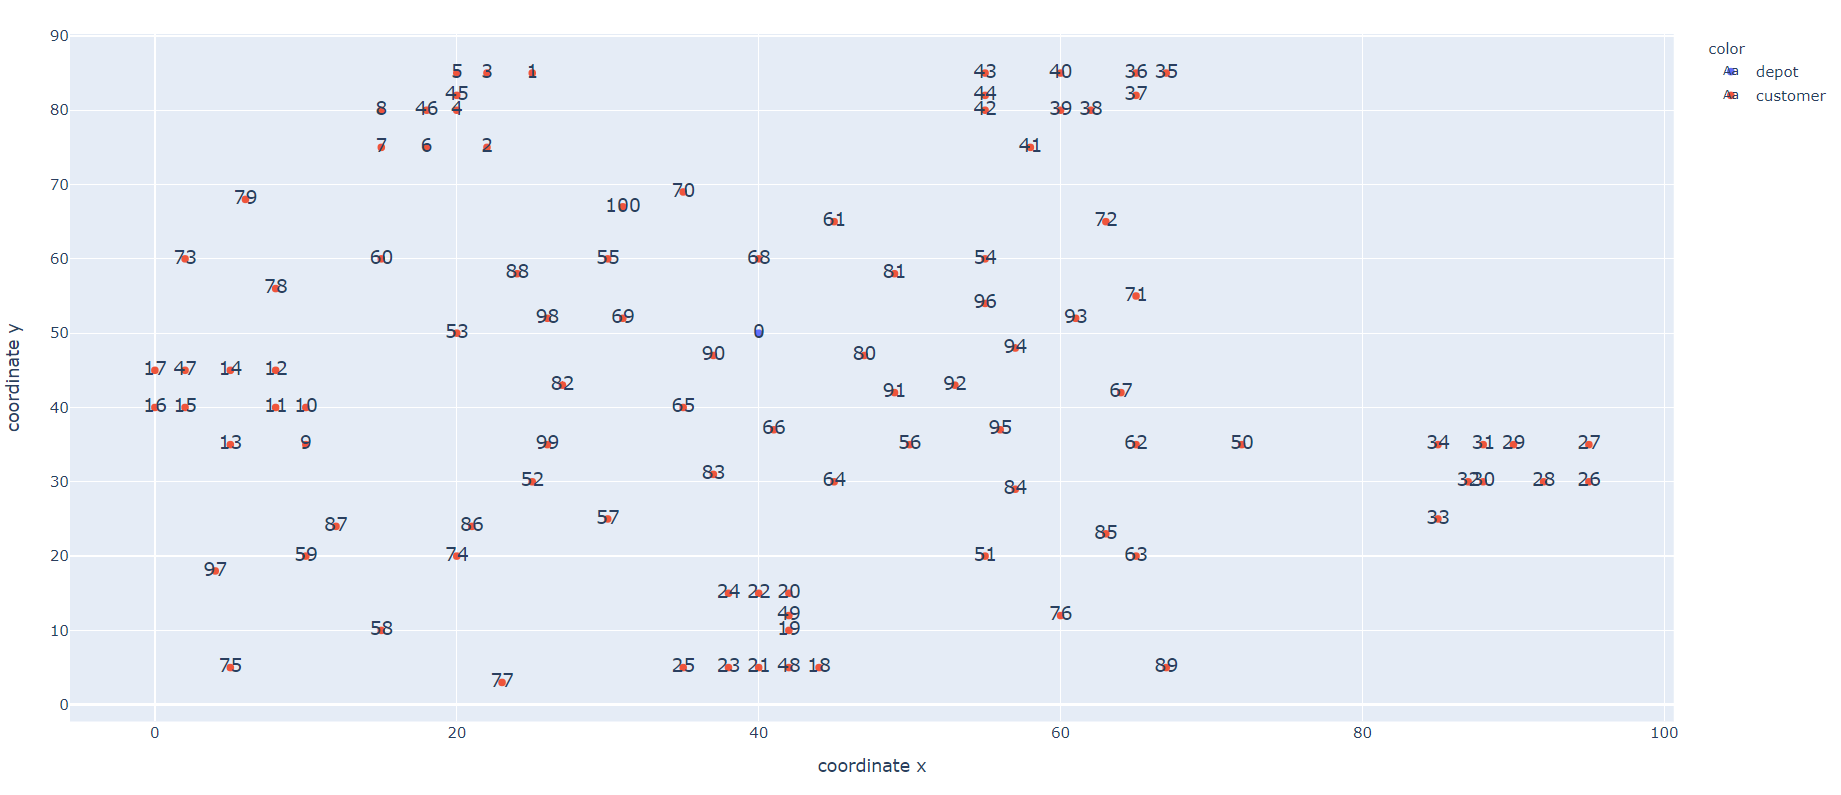
\includegraphics[width=\linewidth]{./img/aumman.png}
	\caption{Map of customers and depot}
	\label{map}
\end{figure}\

However, the customer may prefer a cost allocations which distributes cost equally. The Equal Profit Method and the Lorenz allocation were used to propose two different allocations. Table \ref{EPM} gathers the cost allocation computed with the Equal Profit Method, which took 6 second to be computed. The average cost for each customer is 16.94 money units and the EPM varies from 8.49 to 37.39 and its standard deviation is 6.07. Table \ref{Lorenz} shows the cost allocations computed with Lorenz allocation, which took 7 second to find a solution. This allocation varies from to and its standard deviation is 4.42.

To sum up, three allocation rules were considered to distribute the cost of these fictitious example. It turns out that the Aumann-Dr\`eze's value is the one which takes longer to compute and that it allocates cost based on the distance between customers and the depot. On the other hand, both EPM and Lorenz allocations take less time to compute and they distribute the cost equally. In these example the Lorenz allocation in the one which divides cost more equally between customers.
\clearpage
\begin{table}[H]
	\centering
	\begin{tabular}{c| c |c |c |c|c|c|c}
		\hline 
		%	\centering		
		$i$ customer & $\alpha_i$ & $i$ customer & $\alpha_i$ & $i$ customer & $\alpha_i$& $i$ customer & $\alpha_i$\\
		\hline
		1 & 15.48 & 2 & 16.14 & 3 & 16.0 & 4 & 14.66 \\
		5 & 21.12 & 6 & 13.54 & 7 & 18.52 & 8 & 15.87 \\
		9 & 13.01 & 10 & 12.27 & 11 & 14.71 & 12 & 14.21 \\
		13 & 14.78 & 14 & 13.72 & 15 & 15.25 & 16 & 16.0 \\
		17 & 15.64 & 18 & 18.53 & 19 & 16.43 & 20 & 14.38 \\
		21 & 23.69 & 22 & 14.36 & 23 & 18.48 & 24 & 18.46 \\
		25 & 23.84 & 26 & 16.05 & 27 & 15.04 & 28 & 14.98 \\
		29 & 2.19 & 30 & 16.43 & 31 & 14.49 & 32 & 16.86 \\
		33 & 27.1 & 34 & 14.72 & 35 & 17.57 & 36 & 17.09 \\
		37 & 16.14 & 38 & 14.79 & 39 & 14.33 & 40 & 16.02 \\
		41 & 28.2 & 42 & 31.3 & 43 & 15.13 & 44 & 14.05 \\
		45 & 19.77 & 46 & 15.12 & 47 & 14.87 & 48 & 23.72 \\
		49 & 15.61 & 50 & 13.67 & 51 & 21.51 & 52 & 15.6 \\
		53 & 31.19 & 54 & 10.83 & 55 & 7.41 & 56 & 21.58 \\
		57 & 16.8 & 58 & 20.69 & 59 & 18.61 & 60 & 17.47 \\
		61 & 14.75 & 62 & 18.7 & 63 & 25.05 & 64 & 12.87 \\
		65 & 4.9 & 66 & 15.6 & 67 & 16.23 & 68 & 5.86 \\
		69 & 5.98 & 70 & 7.81 & 71 & 20.21 & 72 & 21.69 \\
		73 & 25.5 & 74 & 22.5 & 75 & 25.01 & 76 & 22.61 \\
		77 & 37.39 & 78 & 21.13 & 79 & 20.15 & 80 & 10.18 \\
		81 & 14.32 & 82 & 6.48 & 83 & 7.89 & 84 & 17.33 \\
		85 & 22.75 & 86 & 20.1 & 87 & 16.76 & 88 & 11.61 \\
		89 & 27.63 & 90 & 5.08 & 91 & 7.72 & 92 & 9.22 \\
		93 & 12.67 & 94 & 10.28 & 95 & 12.87 & 96 & 9.33 \\
		97 & 21.13 & 98 & 5.49 & 99 & 12.81 & 100 & 7.82 \\
		\hline 
	\end{tabular} \
	\caption{Equal profit method cost allocation per customer}
	\label{EPM}
\end{table}\

\begin{table}[H]
	\centering
	\begin{tabular}{c| c |c |c |c|c|c|c}
		\hline 
		%	\centering		
		$i$ customer & $\alpha_i$ & $i$ customer & $\alpha_i$ & $i$ customer & $\alpha_i$& $i$ customer & $\alpha_i$\\
		\hline
		1 & 12.1 & 2 & 15.57 & 3 & 11.87 & 4 & 11.87 \\
		5 & 15.57 & 6 & 18.08 & 7 & 15.57 & 8 & 20.83 \\
		9 & 13.44 & 10 & 13.44 & 11 & 15.83 & 12 & 15.83 \\
		13 & 13.47 & 14 & 13.44 & 15 & 13.44 & 16 & 13.44 \\
		17 & 13.47 & 18 & 15.09 & 19 & 15.09 & 20 & 15.09 \\
		21 & 22.95 & 22 & 15.09 & 23 & 15.09 & 24 & 22.95 \\
		25 & 22.95 & 26 & 13.46 & 27 & 13.46 & 28 & 13.46 \\
		29 & 13.46 & 30 & 13.46 & 31 & 13.46 & 32 & 13.46 \\
		33 & 26.15 & 34 & 13.46 & 35 & 14.77 & 36 & 14.77 \\
		37 & 14.77 & 38 & 14.77 & 39 & 14.77 & 40 & 14.77 \\
		41 & 28.2 & 42 & 25.5 & 43 & 14.77 & 44 & 14.77 \\
		45 & 15.57 & 46 & 11.87 & 47 & 13.44 & 48 & 22.95 \\
		49 & 15.09 & 50 & 13.46 & 51 & 18.47 & 52 & 14.39 \\
		53 & 31.19 & 54 & 10.78 & 55 & 15.57 & 56 & 14.21 \\
		57 & 16.11 & 58 & 15.83 & 59 & 15.83 & 60 & 16.34 \\
		61 & 20.55 & 62 & 18.47 & 63 & 18.47 & 64 & 14.39 \\
		65 & 15.83 & 66 & 19.56 & 67 & 18.47 & 68 & 15.57 \\
		69 & 16.34 & 70 & 14.77 & 71 & 20.21 & 72 & 21.69 \\
		73 & 16.34 & 74 & 20.31 & 75 & 15.83 & 76 & 22.95 \\
		77 & 37.39 & 78 & 16.34 & 79 & 15.57 & 80 & 13.46 \\
		81 & 14.32 & 82 & 15.83 & 83 & 15.09 & 84 & 18.47 \\
		85 & 18.47 & 86 & 14.39 & 87 & 15.83 & 88 & 16.34 \\
		89 & 26.15 & 90 & 8.49 & 91 & 18.47 & 92 & 14.39 \\
		93 & 10.78 & 94 & 10.78 & 95 & 14.39 & 96 & 10.78 \\
		97 & 15.83 & 98 & 13.44 & 99 & 14.39 & 100 & 11.87	\\	
		\hline 
	\end{tabular} \
	\caption{Lorenz allocation per customer}
	\label{Lorenz}
\end{table}\

